\documentclass{article}

\usepackage[defaultposition=I,defaultshowposbase=true]{akkoorden}

\usepackage[margin=.2in]{geometry}

\usepackage{tabu}

\usepackage{xfrac}

\begin{document}

% \akkoord[-]{,x,x/i1,o,o/i2,-}{-}

% \akkoord[-]{-/i3,1,2/1,3/2/i4,4/-/i5,1/1/1}{-}

\begin{tabu}{ X[1,c,m] | X[6,l,m] | X[6,l,m] }
  \textbf{chord} & \textbf{root 6} & \textbf{root 5} \\ \hline
  \textbf{6} &
  \akkoord{}{}
  \akkoord[p=I]{3/2/1,x,2/1/6,4/4/3,3/3/5,x}{G\textsubscript{6}}
  \akkoord[position=II]{2/T/1,4/2/5,4/2/1,3/1/3,4/3/6,4/3/9}{G\textsubscript{69}} &
  \akkoord{x,3/4/1,2/3/3,2/2/6,1/1/1,x}{C\textsubscript{6}}
  \akkoord{3/2/5,3/2/1,2/1/3,2/1/6,3/3/9,3/3/5}{C\textsubscript{69}} \\ \hline
  \textbf{m6 \newline -6} &
  \akkoord{3/1/1,x,2/2/6,3/3/{$\flat$3},3/4/5,x}{G-\textsubscript{6}}
  \akkoord[p=II]{2/T/1,4/2/5,4/2/1,2/1/{$\flat$3},4/3/6,4/3/9}{G-\textsubscript{69}} &
  \\ \hline
  \textbf{Maj7 \newline $\triangle$} &
  \akkoord[p=II]{2/1/1,x,3/3/{$\sharp$7},3/4/3,2/2/5,x}{G\textsubscript{$\triangle$}} &
  \akkoord[p=II]{x,2/1/1,4/3/5,3/2/{$\sharp$7},4/4/3,x}{C\textsubscript{$\triangle$}} \\ \hline
  \textbf{7} &
  \akkoord[p=II]{2/1/1,x,2/2/7,3/4/3,2/3/5,x}{G\textsubscript{7}}
  \akkoord{3/2/1,2/1/3,3/3/7,4/4/3,x,x}{G\textsubscript{7}}
  \akkoord{3/2/1,x,3/3/7,1/1/{$\flat$9},3/4/5,x}{G\textsubscript{7$\flat$9}} &
  \akkoord[p=II]{x,2/1/1,4/3/5,2/1/7,4/4/3,2/1/{(5)}}{C\textsubscript{7}}
  \akkoord{x,3/3/1,2/2/3,3/4/7,1/1/1,x}{C\textsubscript{7}}
  \akkoord{x,3/2/1,2/1/3,3/3/7,3/4/9,3/4/{(5)}}{C\textsubscript{79}} \\ \hline
  \textbf{m7\newline-7} &
  \akkoord[p=II]{2/2/1,x,2/3/7,2/3/{$\flat$3},2/3/5,x}{G-\textsubscript{7}} &
  \akkoord[p=II]{x,2/1/1,4/3/5,2/1/7,3/2/{$\flat$3},2/1/{(5)}}{C-\textsubscript{7}}
  \akkoord{x,3/2/1,1/1/{$\flat$3},3/3/7,4/4/{$\flat$3},x}{C-\textsubscript{7}} \\ \hline
  \textbf{-7$\flat$5 m7$\flat$5 \o \newline halfdim.} &
  \akkoord{3/2/1,x,3/3/7,3/4/{$\flat$3},2/1/{$\flat$5},x}{G\textsubscript{\o}} &
  \akkoord[p=II]{x,2/1/1,3/3/{$\flat$5},2/2/7,3/4/{$\flat$3},x}{C\textsubscript{\o}} \\ \hline
  \textbf{o dim.} \textit{\tiny all notes root, all dist. 1\sfrac{1}{2}} &
  \akkoord{3/2/1,x,2/1/{$\flat$7},3/3/{$\flat$3},2/1/{$\flat$5},x}{G\textsubscript{o}} &
  \akkoord{x,3/2/1,4/3/{$\flat$5},2/1/{$\flat$7},4/4/{$\flat$3},x}{C\textsubscript{o}} \\ \hline \hline
  chord progression ("trap") &
  \begin{tabu}{X[r] X[l]}
    \multicolumn{2}{c}{scale of G: G A B C D E F$\sharp$} \\
    I & G\textsubscript{$\triangle$} \\
    II & A-\textsubscript{7} \\
    III & B-\textsubscript{7} \\
    IV & C\textsubscript{$\triangle$} \\
    V & D\textsubscript{7} \\
    VI & E-\textsubscript{7} \\
    VII & F$\sharp$\textsubscript{o} \\
  \end{tabu} &
  \begin{tabu}{X[r] X[l]}
    \multicolumn{2}{c}{scale of C: C D E F G A B} \\
    I & C\textsubscript{$\triangle$} \\
    II & D-\textsubscript{7} \\
    III & E-\textsubscript{7} \\
    IV & F\textsubscript{$\triangle$} \\
    V & G\textsubscript{7} \\
    VI & A-\textsubscript{7} \\
    VII & B\textsubscript{o} \\
  \end{tabu} \\ \hline
\end{tabu}

\begin{center}
circle of fifths ("kwintencirkel")

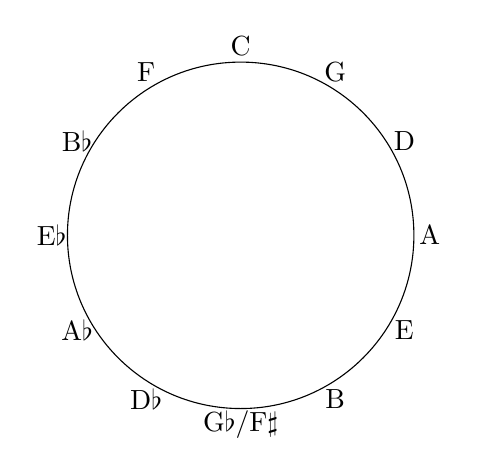
\begin{tikzpicture}
  \draw (0,0) circle [radius=2.2];
  \foreach \x [count=\i,evaluate=\i as \angle using 90-(\i-1)*30] in {C,G,D,A,E,B,{G$\flat$/F$\sharp$},{D$\flat$},{A$\flat$},{E$\flat$},{B$\flat$},F} {
  % \filldraw[fill=white] (\angle:2.7) circle [radius=.45];
  \draw (\angle:2.4) node {\x};
  }
\end{tikzpicture}
\end{center}
\end{document}
